\documentclass[12pt]{article}
\usepackage{geometry} 
\geometry{margin=1in}
\geometry{a4paper} 


\usepackage{textcomp}
\usepackage{booktabs}
\usepackage{array}
\usepackage{paralist}
\usepackage{verbatim} 
\usepackage{subfigure}
\usepackage{graphicx,caption}
\usepackage{placeins}
\usepackage{lipsum}
\usepackage{xcolor}
\usepackage{dcolumn}
\usepackage{sectsty}
\allsectionsfont{\sffamily\mdseries\upshape}
\usepackage{gensymb,amsmath,mathtools,amssymb}
\usepackage{flafter}
%\usepackage{parskip}
\usepackage[utf8]{inputenc}
\usepackage[english]{babel}
\usepackage{tocbibind}
\usepackage[toc,page]{appendix}
\captionsetup{width=\linewidth}
\usepackage{bm}
\usepackage{lscape}


\graphicspath{{./figs/}}


\title{First Order Optimal Sizing of Ascent Vehicles}
\author{Devansh Agrawal}
%\date{} 


\begin{document}

\maketitle


\section{Problem Description}

In designing a ascent vehicle, it is important to start a design relatively close to the optimal solution. In this document, I optimize the thrust of a one dimensional rocket to maximise the apogee altitude. The parameters that are specified fall into the following categories:
\begin{itemize}
\item Environment parameters: $g, \rho(h)$
\item Design parameters: $m_0, m_p, c_d, A,c$\footnote{$m_0$ is the launch mass, $m_p$ is the propellant mass}
\item Control parameters: $F(t)$
\end{itemize}

For initial sizing, we make the following assumptions on the rocket dynamics:
\begin{itemize}
\item Earth is inertial, non-rotating, and the acceleration due to gravity is constant with altitude, $g = 9.81$~m/s$^2$
\item Earths atmosphere follows an exponential relationship, $\rho(h) = \rho_0 e^{-\beta h}$, where for the earth, $\rho_0 = 1.225$~kg/m$^3$, $\beta = 1/8.5$~km$^{-1}$
\item The rockets drag coefficient is constant, independent of the mach number\footnote{In general, this is not a good assumption, however, as we will see later, the maximum mach number of the rocket is to be kept below $M\sim0.7$. A numeric optimiser should be used later to refine the vehicle.}
\item The rockets specific impulse is a constant $I_{sp} = c g_0$, and does not depend on altitude.
\item The thrust curve is extremely simple. The rocket thrusts at a constant $F$~newtons for $t_b$~seconds. For this simplifying case, we do not need to include $t_b$ in our parameters since it is implicitly defined:
\begin{align}
I_t &= \int F dt = F t_b\\
\text{and } I_t &= \int -\dot{m} c dt  = m_p c\\
\therefore t_b &= \frac{m_p c}{F}
\end{align}
\end{itemize}


Hence, we will try to determine the optimum value of $F$ given all the other parameters. 

\section{State space description, and non-dimensionalisation}

The dynamics of a 1-D rocket can be written as
\begin{align} 
\dot{h} &=v \\
\dot{v} &=\frac{1}{m}(F(t)-D(v, h))-g \\
\dot{m} &=\frac{-F(t)}{c} 
\end{align}

Directly integrating this is difficult, but we can do so numerically, using Mathematica. From their, the maximum height is readily determined. However there are 6 parameters that can be chosen in this problem, and the dependence due to 3 more. To simplify the analysis we introduce non-dimensional parameters. The reference quantities used are

\begin{itemize}
\item Mass: $m_0$
\item Acceleration: $g$
\item Speed: $c$
\end{itemize}

Therefore the following reference dimensions can be found:
\begin{itemize}
\item Force: $m_0 g$
\item Time: $c/g$
\item Length: $c^2/g$
\item Total Impulse: $1/(m_0 c)$
\end{itemize}

Using hats to denote the non-dimensionalised quantities, the state space equation can be written as 

\begin{align}
\dot{\hat{h}} &=\hat{v} \\
\dot{\hat v} &=\frac{\hat F}{\hat m}  - \left( \frac{\rho c^2 c_d A}{2 m_0 g} \right) e^{- (\beta c^2/g) \hat h}  \frac{ \hat{v}^2}{\hat m}  - 1 \\
\dot{\hat m} &=-\hat F
\end{align}

Furthermore, the switching occurs at $t = t_b$. Interestingly, the non-dimensionalized total impulse is  directly related to the propellant mass fraction:
\begin{align}
\hat{I_t} &= \frac{I_t}{m_0 c} = \frac{F t_b}{m_0 c} = \frac{m_p c}{m_0 c} = \frac{m_p}{m_0}\\
\therefore \hat{t_b} &= \frac{I_t}{F} = \frac{m_p}{m_0} \frac{1}{\hat F}
\end{align}

Therefore, the important parameters are now immediately obvious, and can be interpreted as,

\begin{enumerate}
\item The thrust to initial weight ratio, 
\begin{equation}
\hat F = \frac{F}{m_0 g}
\end{equation}

\item A drag parameter defined as,
\begin{equation}
x \equiv \frac{\frac{1}{2} \rho c^2 c_d A}{m_0 g}
\end{equation}
Note: This parameter is like the drag to weight ratio (except it uses $c$ as the velocity and $m_0$ as the mass)

\item Propellant mass fraction,
\begin{equation}
MR \equiv m_p/m_0
\end{equation}

\item Atmosphere parameter, 
\begin{equation}
\hat \beta = \beta \frac{c^2}{g}
\end{equation}
which scales the atmosphere's height to the height we are interested in. 
\end{enumerate}

Finally, the parameter to be optimised is the final altitude, 

\begin{equation}
h_f = \hat h_f \frac{c^2}{g}
\end{equation} 


Therefore, our 8 parameter space has reduced to a four parameter space, three if we assume the specific impulse of the rocket is fixed.

The typical range of these parameters, and a rough order of magnitude for a 10k solid rocket are

\begin{center}
   \begin{tabular}{@{} ccc@{}}
      \toprule
      Parameter & Typical value & Range\\
      \midrule
      $\hat F$ & 15 & $>1$\\
      $x$ & 60 & $>0$\\
      $MR$ & 0.15 & $0.3\sim0.9$\\
      $\hat \beta$ & 50 & $25 \sim 75$\\
      $\hat h_f$ & 0.0075 \\
      \bottomrule
   \end{tabular}
\end{center}
where the $\hat h_f = 0.0075$  is the value that corresponds to 10k ft. 

Note, while the thrust to weight ratio is approximately 15 for rockets for IREC, most big rockets have $\hat F$ closer to 1.5! The next section shows this is actually very close to the optimum.


\section{Optimization Results}

A relatively brute force form of optimisation is attempted, in the interest of time. A Mathematica function is written to solve the dynamics equations, given the four parameters. The apogee height is returned by this function. The numerical schemes used are Mathematica's 'automatic' choices, which generally performs well, even through stiff systems. Since the problem is initial valued, it is fairly trivial to solve numerically. 

A few simulated trajectories are shown below, as samples. It is hard to believe that these are optimally sized vehicles. 

%\FloatBarrier
\begin{figure}[htbp]
   \centering
   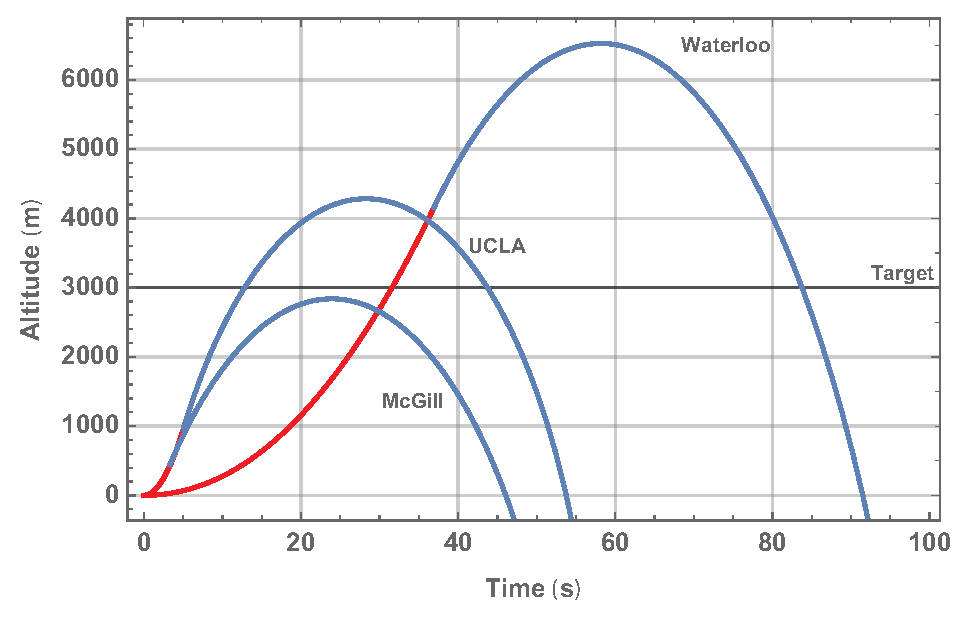
\includegraphics[width=0.8\linewidth]{sample_flights.eps}
   \caption{Sample simulated flights based on data from 2018 reports. Red indicates thrusting, blue indicates coasting.}
   
      \begin{tabular}{@{} llcccc|ccc@{}}
         \toprule
         Team &Type & $C_D$ (est) & $c$ (m/s, assumed) & dia (in) & $m_0$ (kg) &  $x$ & $m_p/m_0$ & $T/W$ \\ 
         \midrule
         McGill & Solid & 0.5 & 2000 & 5 & 24 & 64.6 &0.146 & 8.8\\
         Waterloo& Hybrid & 0.5 & 2000 & 6 & 64.8 & 34.48 &0.280 & 1.5\\
         UCLA & Hybrid &0.5 & 2000 & 6 & 26.7 & 83.7 & 0.21 & 8.5\\
         \bottomrule
      \end{tabular}
    \label{fig:}
\end{figure}
%FloatBarrier


Now we can see the trade between thrust to weight ratio and propellant mass fraction. 

\begin{landscape}
%\FloatBarrier
\begin{figure}[htbp]
   \centering
   \includegraphics[width=\linewidth]{Tw-MR_contours.eps}
   \caption{}
   \label{fig:}
\end{figure}
%FloatBarrier
\end{landscape}


The red line indicates the 10k target altitude (assuming $c = 2000~m/s$). This shows that for a range of $x$, the easiest to design scenarios are for T/W>3, and propellant mass fraction around 15\%. Below a thrust to weight ratio of 2, the height is very sensitive to the propellant mass fraction. 

It is also interesting to see that as the propellant mass fraction increases, it becomes better to reduce thrust to weight ratio towards T/W $\sim$ 2. 


Ultimately however, we need to find a design that can achieve the desired altitude, while minimising the total mass and thrust level required. If we limit max thrust to 1~kN, and assume $c=2000$~m/s and $c_d = 0.5$, we can figure out possible designs:

%\FloatBarrier
\begin{figure}[htbp]
   \centering
   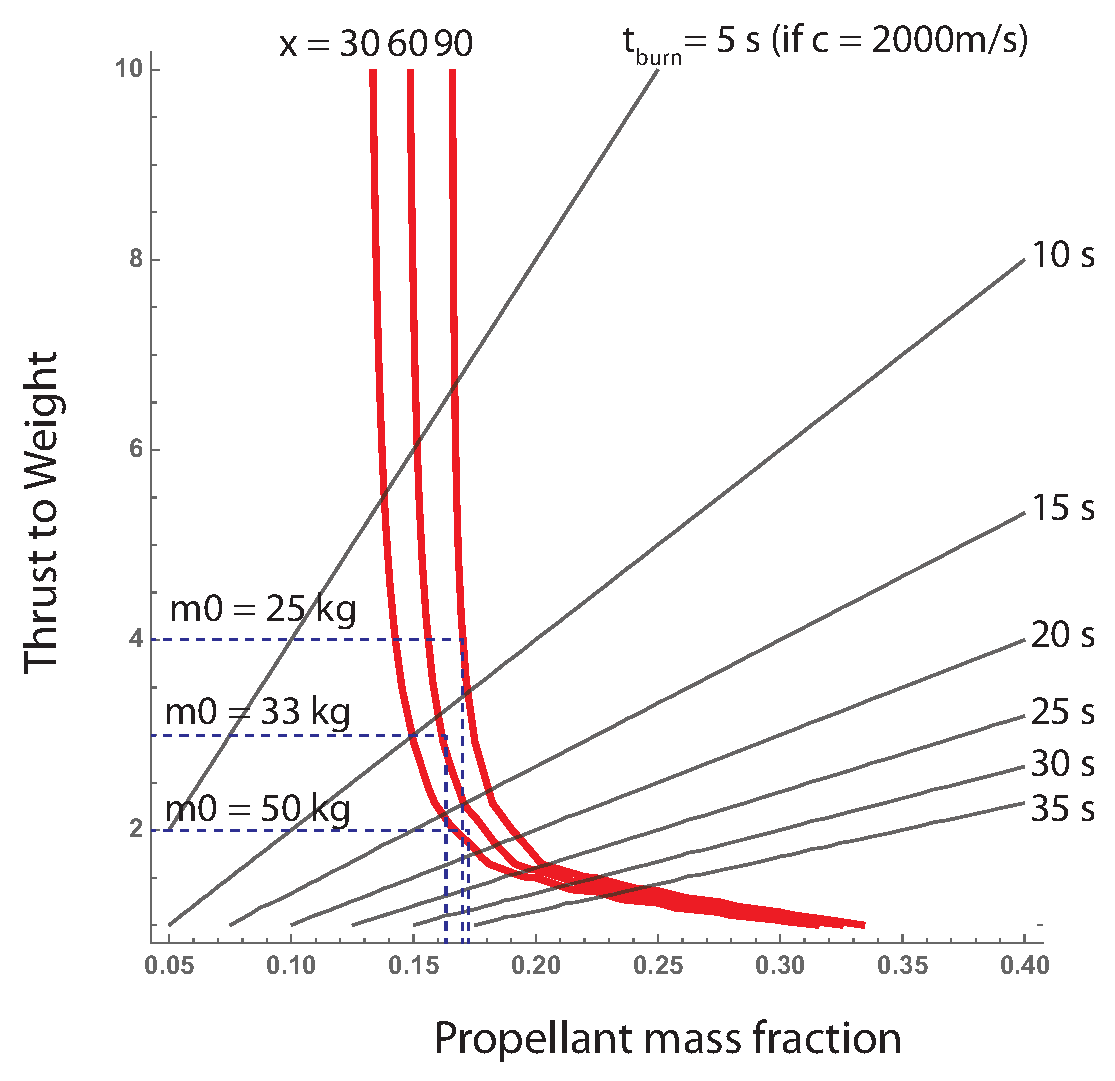
\includegraphics[width=0.8\linewidth]{results.eps}
   \caption{}
   \label{fig:}
\end{figure}
%FloatBarrier

This figure shows the required propellant mass fraction is about 17\%, over a range of vehicle masses. It is obvious that reducing the vehicles mass would be beneficial, as it gives more flexibility in the future, and increases the acceleration, and therefore stability, but is also important for the propellant mass fraction to be as close to 17\% as possible. 

Why is there such a steep slope to the graphs? One way to think about it is as follows. For very large thrust to weight, the rocket burns very rapidly, and acts as impulse. From there, the vehicle is basically passive, and the ratio of drag to inertia (the parameter $x$) controls the final altitude. Therefore in the limit that thrust to weight becomes large, 


\end{document}























